\documentclass{exos}
\usepackage{main}

\begin{document}
Soit $ABCD$ un rectangle tel que $AB = 4$ et $AD = 10$. Soit $M$ un point quelconque du segment $[BC]$. Où placer le point $M$ sur le segment $[BC]$ pour que le triangle $AMD$ soit rectangle en $M$ ?
\begin{center}
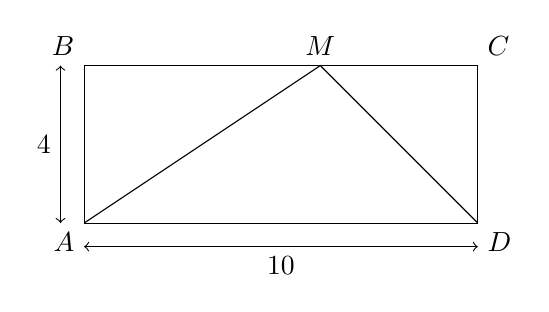
\begin{tikzpicture}
\coordinate (A) at (0,0);
\coordinate (B) at (0,2);
\coordinate (C) at (5,2);
\coordinate (D) at (5,0);
\coordinate (M) at (3,2);

\draw (A) -- (B) -- (C) -- (D) -- cycle;
\draw (A) -- (M) -- (D);
\draw (A) node[below left] {$A$};
\draw (B) node[above left] {$B$};
\draw (C) node[above right] {$C$};
\draw (D) node[below right] {$D$};
\draw (M) node[above] {$M$};
\draw [<->] ([yshift=-0.3cm]A) -- ([yshift=-0.3cm]D) node[midway,below] {$10$};
\draw [<->] ([xshift=-0.3cm]A) -- ([xshift=-0.3cm]B) node[midway,left] {$4$};
\end{tikzpicture}
\end{center}
\vspace*{2cm}
Soit $ABCD$ un rectangle tel que $AB = 4$ et $AD = 10$. Soit $M$ un point quelconque du segment $[BC]$. Où placer le point $M$ sur le segment $[BC]$ pour que le triangle $AMD$ soit rectangle en $M$ ?
\begin{center}
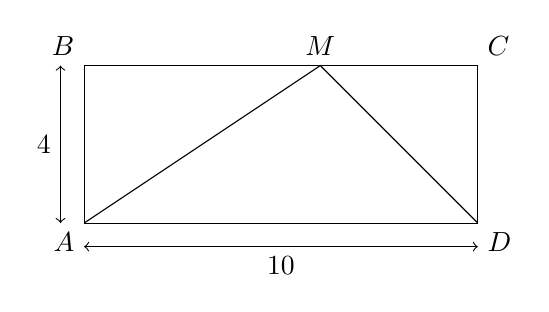
\begin{tikzpicture}
\coordinate (A) at (0,0);
\coordinate (B) at (0,2);
\coordinate (C) at (5,2);
\coordinate (D) at (5,0);
\coordinate (M) at (3,2);

\draw (A) -- (B) -- (C) -- (D) -- cycle;
\draw (A) -- (M) -- (D);
\draw (A) node[below left] {$A$};
\draw (B) node[above left] {$B$};
\draw (C) node[above right] {$C$};
\draw (D) node[below right] {$D$};
\draw (M) node[above] {$M$};
\draw [<->] ([yshift=-0.3cm]A) -- ([yshift=-0.3cm]D) node[midway,below] {$10$};
\draw [<->] ([xshift=-0.3cm]A) -- ([xshift=-0.3cm]B) node[midway,left] {$4$};
\end{tikzpicture}
\end{center}
\vspace*{2cm}
Soit $ABCD$ un rectangle tel que $AB = 4$ et $AD = 10$. Soit $M$ un point quelconque du segment $[BC]$. Où placer le point $M$ sur le segment $[BC]$ pour que le triangle $AMD$ soit rectangle en $M$ ?
\begin{center}
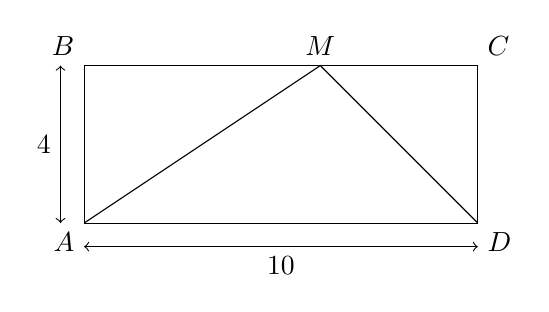
\begin{tikzpicture}
\coordinate (A) at (0,0);
\coordinate (B) at (0,2);
\coordinate (C) at (5,2);
\coordinate (D) at (5,0);
\coordinate (M) at (3,2);

\draw (A) -- (B) -- (C) -- (D) -- cycle;
\draw (A) -- (M) -- (D);
\draw (A) node[below left] {$A$};
\draw (B) node[above left] {$B$};
\draw (C) node[above right] {$C$};
\draw (D) node[below right] {$D$};
\draw (M) node[above] {$M$};
\draw [<->] ([yshift=-0.3cm]A) -- ([yshift=-0.3cm]D) node[midway,below] {$10$};
\draw [<->] ([xshift=-0.3cm]A) -- ([xshift=-0.3cm]B) node[midway,left] {$4$};
\end{tikzpicture}
\end{center}
\vspace*{2cm}
Soit $ABCD$ un rectangle tel que $AB = 4$ et $AD = 10$. Soit $M$ un point quelconque du segment $[BC]$. Où placer le point $M$ sur le segment $[BC]$ pour que le triangle $AMD$ soit rectangle en $M$ ?
\begin{center}
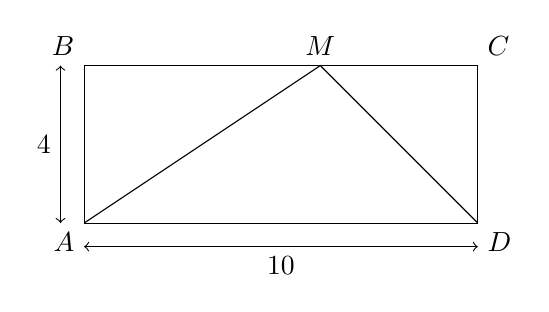
\begin{tikzpicture}
\coordinate (A) at (0,0);
\coordinate (B) at (0,2);
\coordinate (C) at (5,2);
\coordinate (D) at (5,0);
\coordinate (M) at (3,2);

\draw (A) -- (B) -- (C) -- (D) -- cycle;
\draw (A) -- (M) -- (D);
\draw (A) node[below left] {$A$};
\draw (B) node[above left] {$B$};
\draw (C) node[above right] {$C$};
\draw (D) node[below right] {$D$};
\draw (M) node[above] {$M$};
\draw [<->] ([yshift=-0.3cm]A) -- ([yshift=-0.3cm]D) node[midway,below] {$10$};
\draw [<->] ([xshift=-0.3cm]A) -- ([xshift=-0.3cm]B) node[midway,left] {$4$};
\end{tikzpicture}
\end{center}
\end{document}